\documentclass{article}
\usepackage[a4paper, total={6in, 8in}]{geometry}
\usepackage{amsmath,amsfonts,amssymb}
\usepackage{graphicx}
\usepackage{cleveref}

% \newcommand{\beginsupplement}{
% 	\setcounter{table}{0}
% 	\renewcommand{\thetable}{S\arabic{table}}
% 	\setcounter{figure}{0}
% 	\renewcommand{\thefigure}{S\arabic{figure}}
% 	\crefname{figure}{Fig. S}{figures S}
% 	 \renewcommand{\figurename}{Supplementary Figure}
% 	 \onecolumn
% }

\begin{document}
% \beginsupplement

\begin{figure}
    \centering
    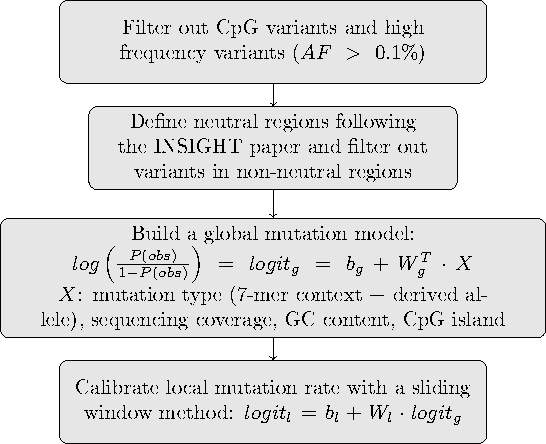
\includegraphics[width=0.8\linewidth]{supplemental_figures/neutral_mutation_model_pipeline.pdf}
    \caption{\textbf{Neutral mutation model pipeline}}
    \label{fig:mutation_model_pipeline}
\end{figure}

\begin{figure}
    \centering
    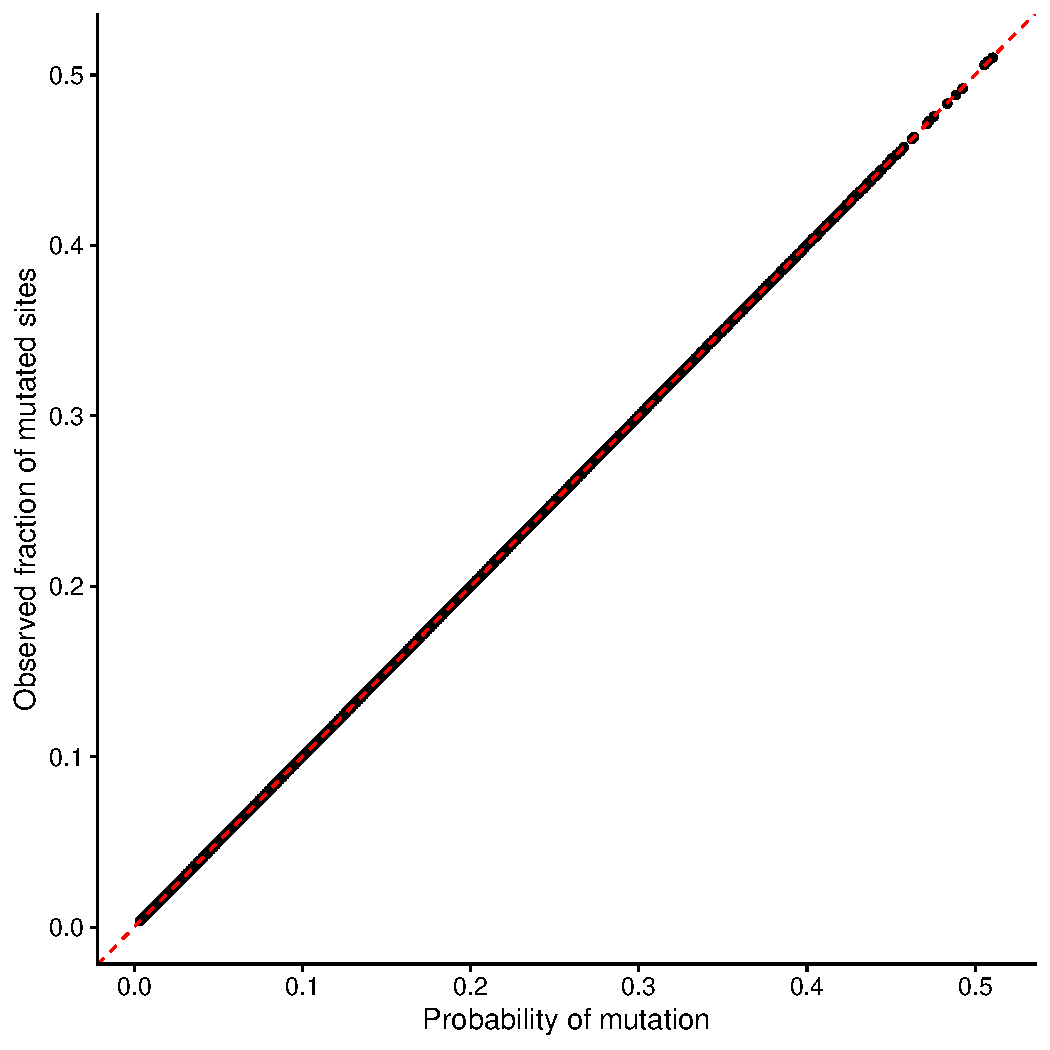
\includegraphics[width = 0.5\linewidth]{supplemental_figures/mutation_model_calibration.pdf}
    \caption{\textbf{The mutation model is globally well calibrated in neutral regions}}
    \label{fig:mutation_model_calibration}
\end{figure}

\begin{figure}
    \centering
    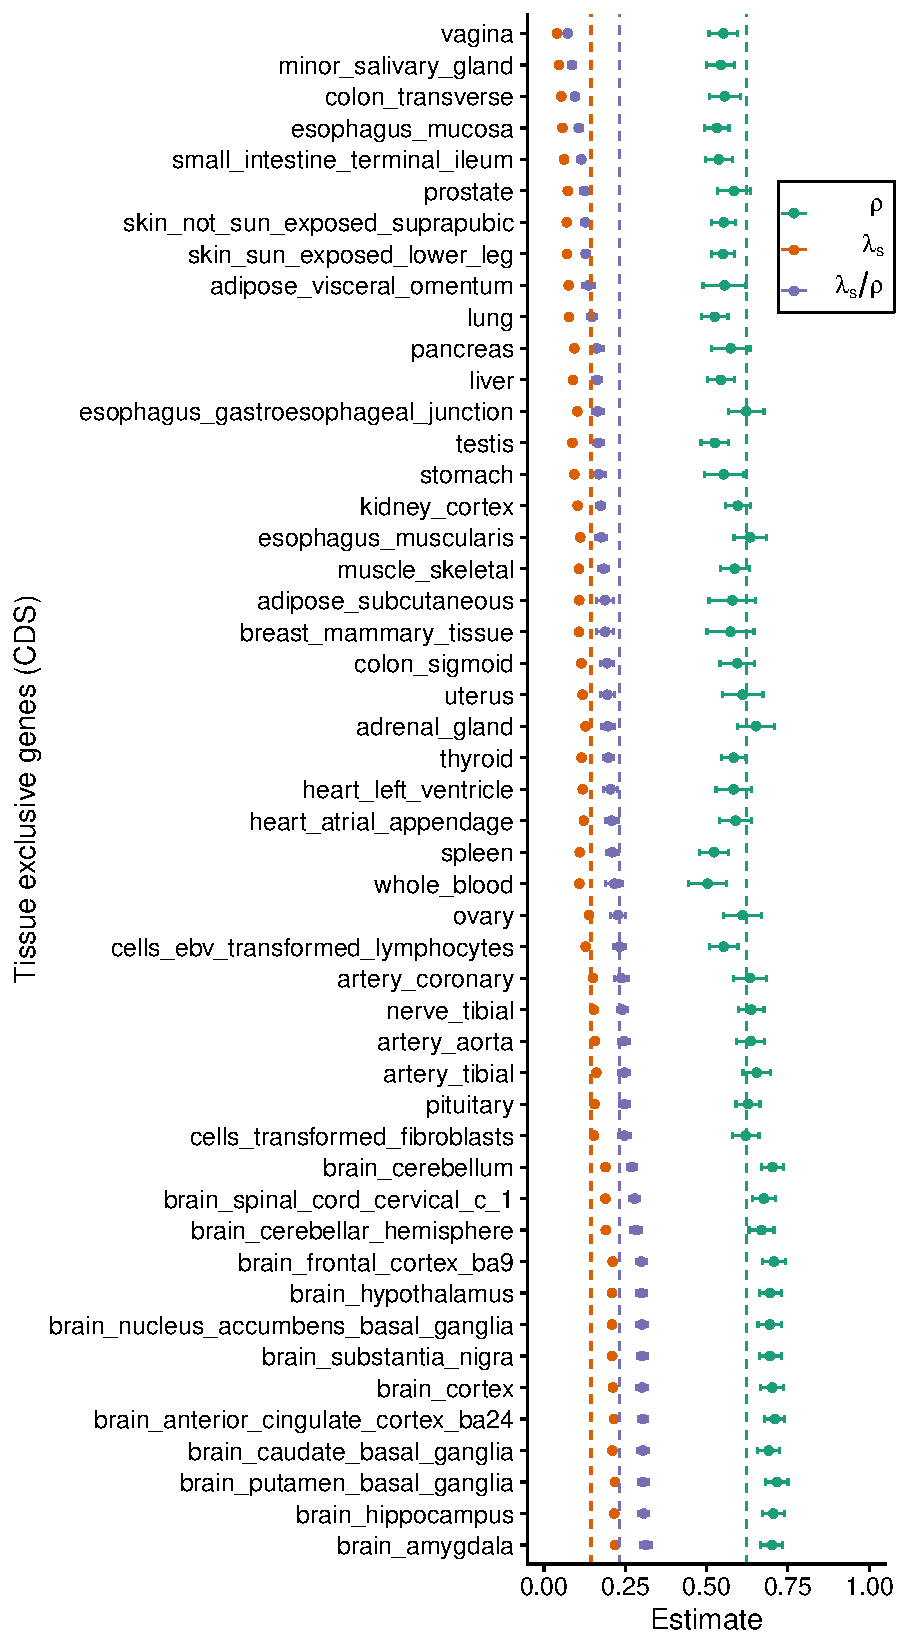
\includegraphics[width = 0.65\linewidth]{supplemental_figures/tissue_specificity_cds_ratio.pdf}
    \caption{\textbf{ExtRaINSIGHT and INSIGHT scores for tissue specific genes}}
    \label{fig:tissue_specific_scores}
\end{figure}

\begin{figure}
    \centering
    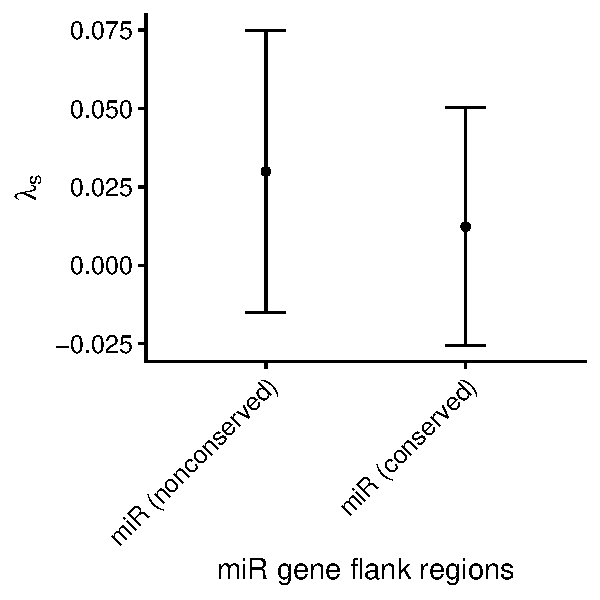
\includegraphics[width = 0.6\linewidth]{supplemental_figures/miRNA_flank_constraint.pdf}
    \caption{\textbf{Excess mutation rates not observed in the regions flanking miRNA genes}}
    \label{fig:miRNA_flank}
\end{figure}

\begin{figure}
    \centering
    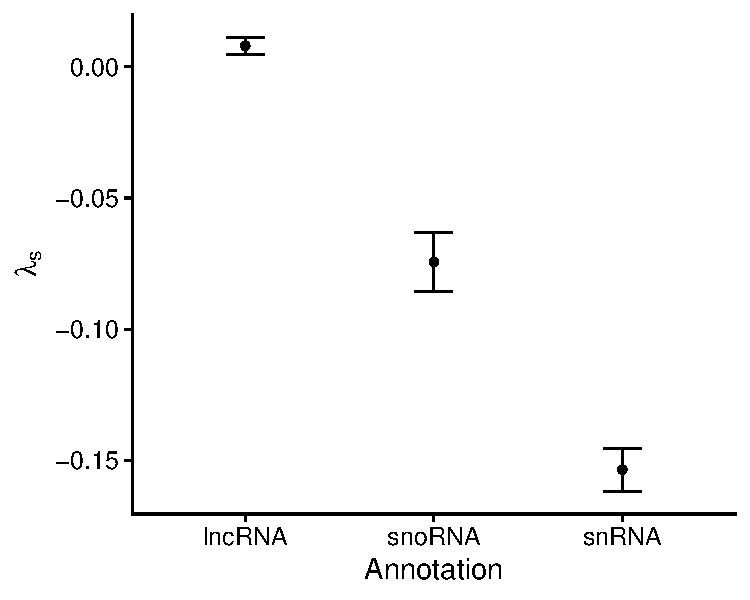
\includegraphics[width = 0.6\linewidth]{supplemental_figures/noncoding_rnas_constraint.pdf}
    \caption{\textbf{Excess mutation rates are observed in some classes of non-coding RNAs}}
    \label{fig:extra_insight_model}
\end{figure}

\end{document}



